% $Header: /cvsroot/latex-beamer/latex-beamer/solutions/conference-talks/conference-ornate-20min.en.tex,v 1.6 2004/10/07 20:53:08 tantau Exp $

\documentclass{beamer}

% This file is a solution template for:

% - Talk at a conference/colloquium.
% - Talk length is about 20min.
% - Style is ornate.



% Copyright 2004 by Till Tantau <tantau@users.sourceforge.net>.
%
% In principle, this file can be redistributed and/or modified under
% the terms of the GNU Public License, version 2.
%
% However, this file is supposed to be a template to be modified
% for your own needs. For this reason, if you use this file as a
% template and not specifically distribute it as part of a another
% package/program, I grant the extra permission to freely copy and
% modify this file as you see fit and even to delete this copyright
% notice. 


\mode<presentation>
{
  \usetheme{Warsaw}
  % or ...

  \setbeamercovered{transparent}
  % or whatever (possibly just delete it)
}


\usepackage[english]{babel}
% or whatever

\usepackage[latin1]{inputenc}
% or whatever

\usepackage{times}
\usepackage[T1]{fontenc}
% Or whatever. Note that the encoding and the font should match. If T1
% does not look nice, try deleting the line with the fontenc.
\usepackage{url}
\usepackage{epstopdf}


\title
{GRID Application Portal}

\author
{Martin Matusiak\inst{1} \and Jonas Lindemann\inst{2}}
% - Give the names in the same order as the appear in the paper.
% - Use the \inst{?} command only if the authors have different
%   affiliation.

\institute
{
  \inst{1}%
  The NTNU High Performance Computing Project\\
  Norwegian University of Science and Technology
  \and
  \inst{2}%
  Lunarc, Center for Scientific and Technical Computing\\
  Lund University}
% - Use the \inst command only if there are several affiliations.
% - Keep it simple, no one is interested in your street address.

\date[1st NGN 2005] % (optional, should be abbreviation of conference name)
{1st Nordic Grid Neighbourhood Conference\\
\footnotesize University of Oslo, Norway, 15-17 August 2005}
% - Either use conference name or its abbreviation.
% - Not really informative to the audience, more for people (including
%   yourself) who are reading the slides online


% Delete this, if you do not want the table of contents to pop up at
% the beginning of each subsection:
\AtBeginSubsection[]
{
  \begin{frame}<beamer>
    \frametitle{Outline}
    \tableofcontents[currentsection,currentsubsection]
  \end{frame}
}


% If you wish to uncover everything in a step-wise fashion, uncomment
% the following command: 

%\beamerdefaultoverlayspecification{<+->}


\begin{document}

\begin{frame}
  \titlepage
\end{frame}

\begin{frame}
  \frametitle{Outline}
  \tableofcontents
  % You might wish to add the option [pausesections]
\end{frame}


% Structuring a talk is a difficult task and the following structure
% may not be suitable. Here are some rules that apply for this
% solution: 

% - Exactly two or three sections (other than the summary).
% - At *most* three subsections per section.
% - Talk about 30s to 2min per frame. So there should be between about
%   15 and 30 frames, all told.

% - A conference audience is likely to know very little of what you
%   are going to talk about. So *simplify*!
% - In a 20min talk, getting the main ideas across is hard
%   enough. Leave out details, even if it means being less precise than
%   you think necessary.
% - If you omit details that are vital to the proof/implementation,
%   just say so once. Everybody will be happy with that.

\section{Motivation}



\subsection{The command line interface}

\begin{frame}
  \frametitle{Introducing the command line interface to Nordugrid}

	\includegraphics[width=\textwidth]{console_submit.png}
\end{frame}

\begin{frame}
  \frametitle{Assessing the command line interface}

	Advantages:
  \begin{itemize}
  	\item Flexible
	  \item Efficient
	  \item Suitable for large data sets
  \end{itemize}
  Conclusion: {\bf Ideal for the "power user"}
	\bigskip
	
  Drawbacks:
  \begin{itemize}
  	\item Intimidating at first sight
	  \item Commands require memorizing
	  \item Not everyone is comfortable with Unix
  \end{itemize}
  Conclusion: {\bf Sub-par for the casual user}
\end{frame}



\subsection{A proposed solution}

\begin{frame}
  \frametitle{A GRID Application Portal}

	A solution proposed by Jonas --\\ the LUNARC Application Portal,
  \begin{itemize}
  	\item offering a web-based interface for simplicity,
  	\item revolving around a work flow model (create job, submit job, monitor job, get job),
  	\item providing a unified interface to applications (adding support for new applications is straightforward),
  	\item without compromising the security model.
  \end{itemize}	
	
\end{frame}

\begin{frame}
  \frametitle{A portal in two flavors}

	LUNARC Application Portal
  \begin{itemize}
  	\item the original codebase
	  \item developed at Lund University by Jonas
  \end{itemize}
	\bigskip
	
  GRIDportal
  \begin{itemize}
  	\item a fork off LUNARC Application Portal
	  \item developed at NTNU by Martin to suit NTNU needs
  \end{itemize}
  \bigskip
  
  In spite of the split, both are moving toward an eventual merge.
\end{frame}



\subsection{The portal interface}

\begin{frame}
  \frametitle{Aims of the portal interface}

	The portal aims to:
  \begin{itemize}
  	\item make GRID computing easy to the "uninitiated" with a minimum of schooling
  	\item conceal the intricate details of GRID computing
  	\item offer a pluggable interface to applications
  \end{itemize}
\end{frame}

\begin{frame}
  \frametitle{Introducing the portal interface to Nordugrid (1/4)}

	\begin{center}
		\includegraphics[width=0.85\textwidth]{portal_submit.png}
	\end{center}
\end{frame}

\begin{frame}
  \frametitle{Introducing the portal interface to Nordugrid (2/4)}

	\begin{center}
		\includegraphics[width=0.85\textwidth]{portal_monitor.png}
	\end{center}	
\end{frame}

\begin{frame}
  \frametitle{Introducing the portal interface to Nordugrid (3/4)}

	\begin{center}
		\includegraphics[width=0.85\textwidth]{portal_get.png}
	\end{center}
\end{frame}

\begin{frame}
  \frametitle{Introducing the portal interface to Nordugrid (4/4)}

	\begin{center}
		\includegraphics[width=0.85\textwidth]{portal_files.png}
	\end{center}	
\end{frame}

\begin{frame}
  \frametitle{Assessing the portal interface}

	Advantages:
  \begin{itemize}
  	\item Intuitive, easy-to-understand interface
	  \item No memorizing necessary, all options are displayed
	  \item Not restricted to Unix, easier for Windows users
  \end{itemize}
  Conclusion: {\bf Ideal for the casual user}?
	\bigskip
	
  Drawbacks:
  \begin{itemize}
  	\item Inflexible (web interface does not provide the full array of command line switches)
	  \item Inefficient with extensive use
	  \item Unsuitable for large data sets (more on this later)
  \end{itemize}
  Conclusion: {\bf Sub-par for the "power user"}
\end{frame}






\section{Design}







\subsection{Relation to Nordugrid/ARC}


\begin{frame}
  \frametitle{The top level perspective}

	\begin{center}
		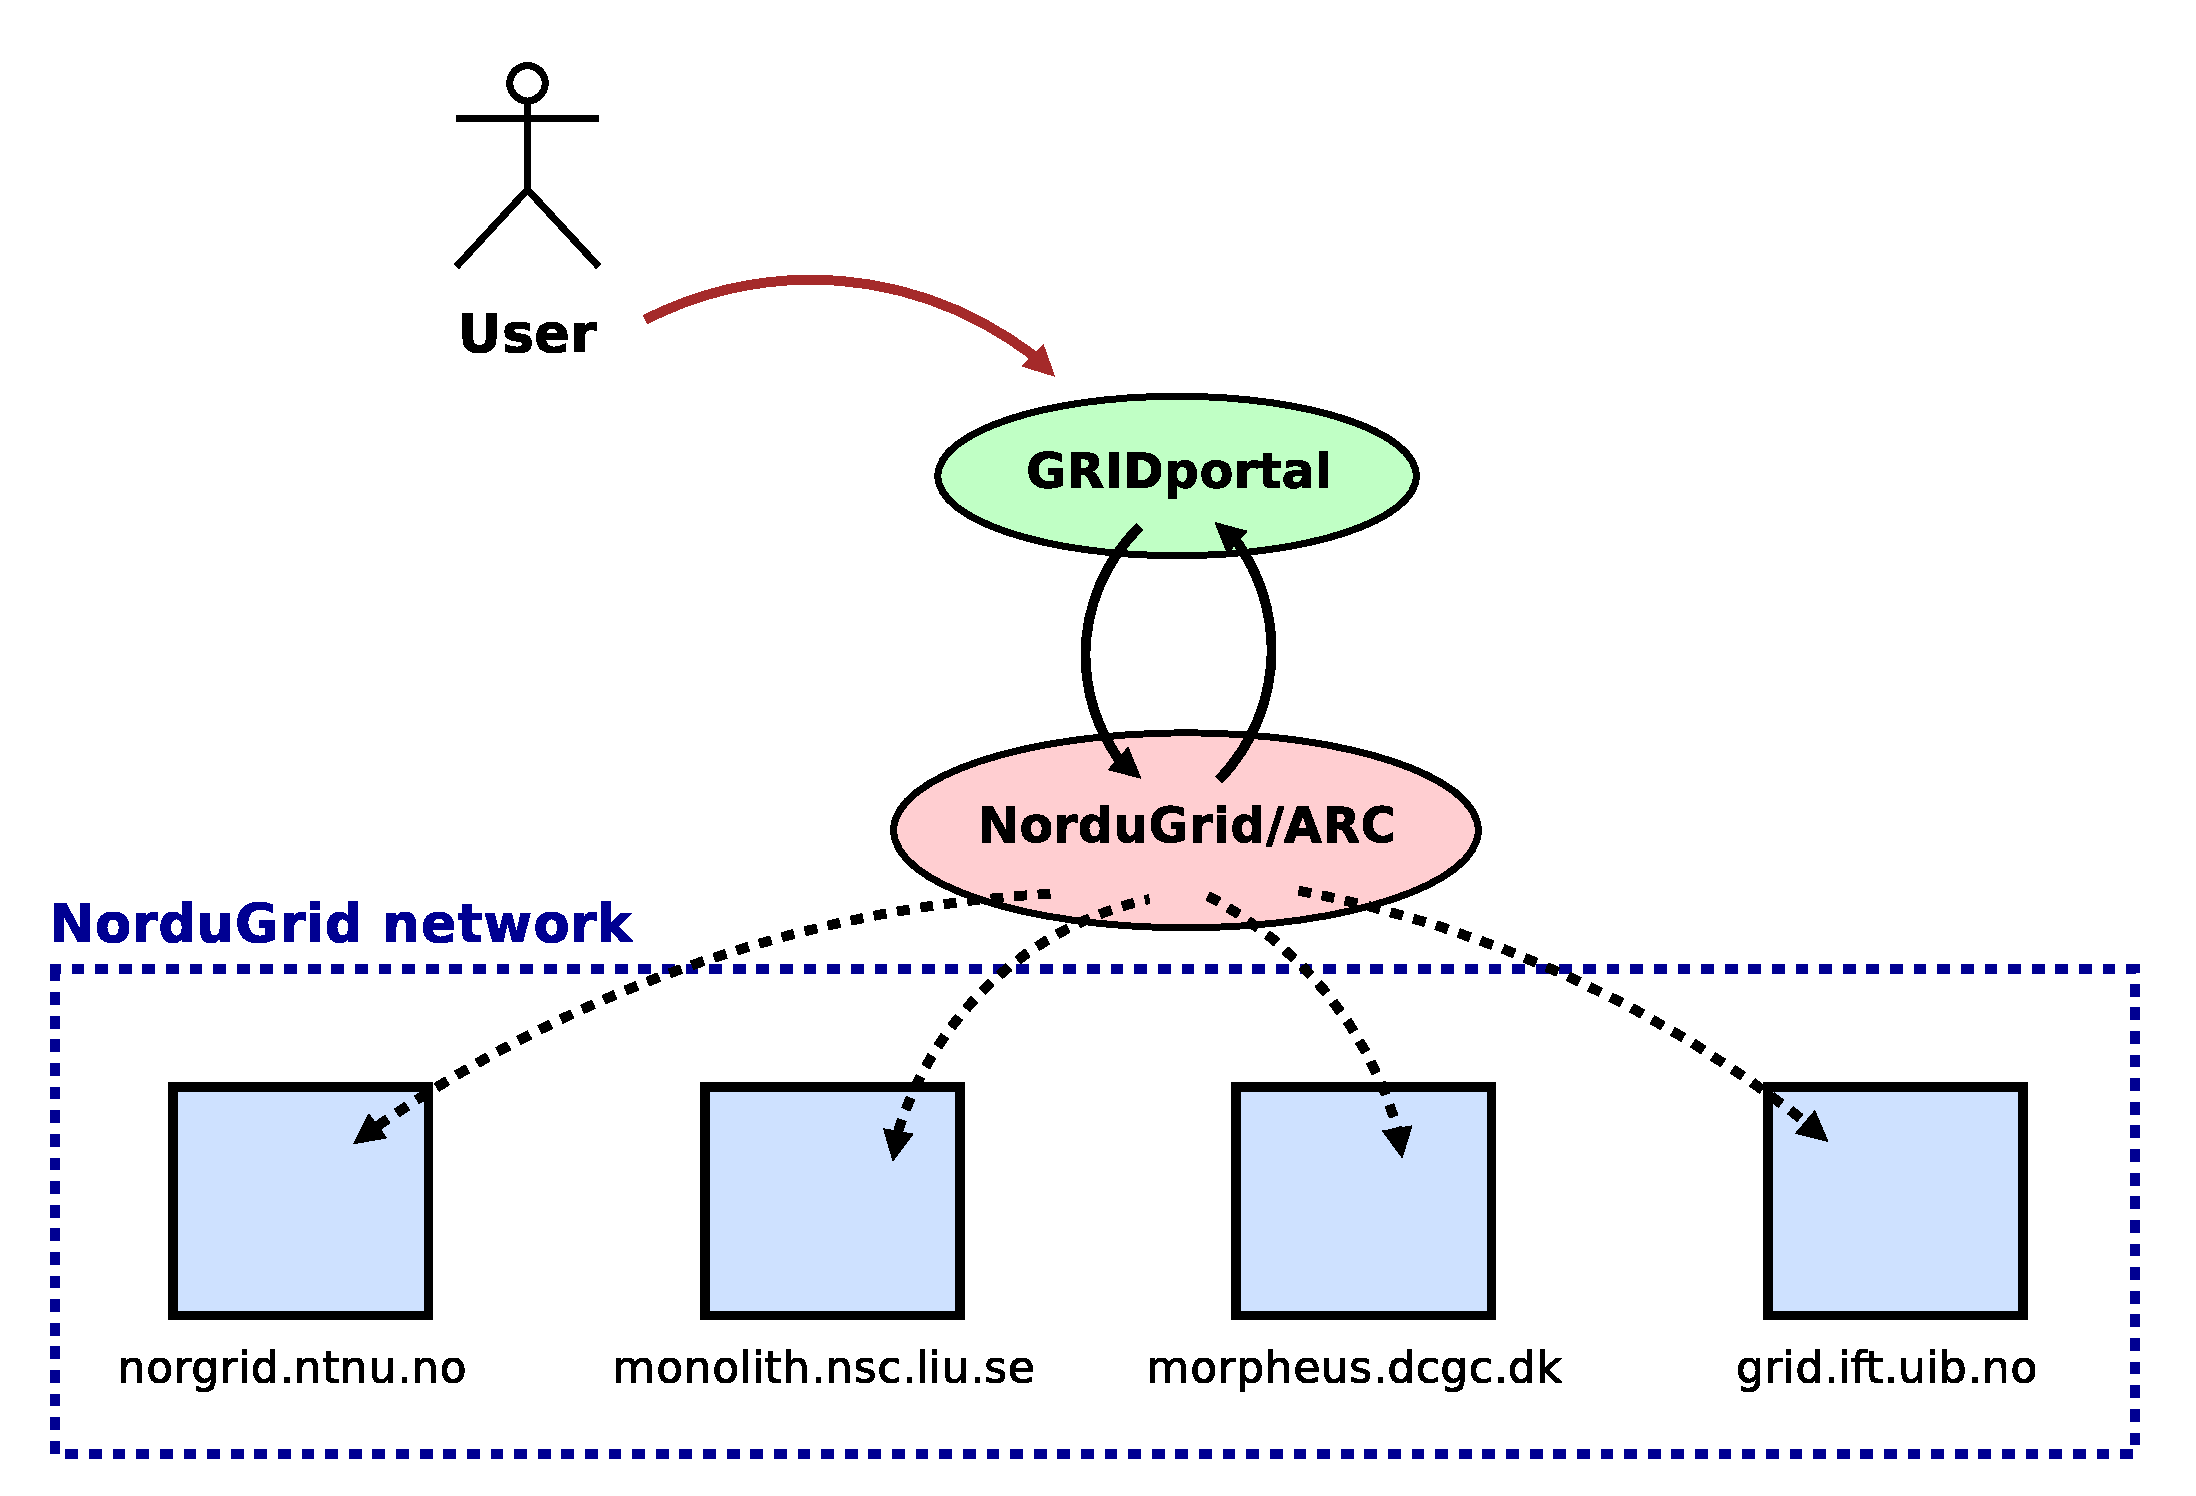
\includegraphics[width=0.8\textwidth]{nordugrid.eps}
	\end{center}	
\end{frame}


\begin{frame}
  \frametitle{A real world example -- norgrid.ntnu.no}

	\begin{center}
		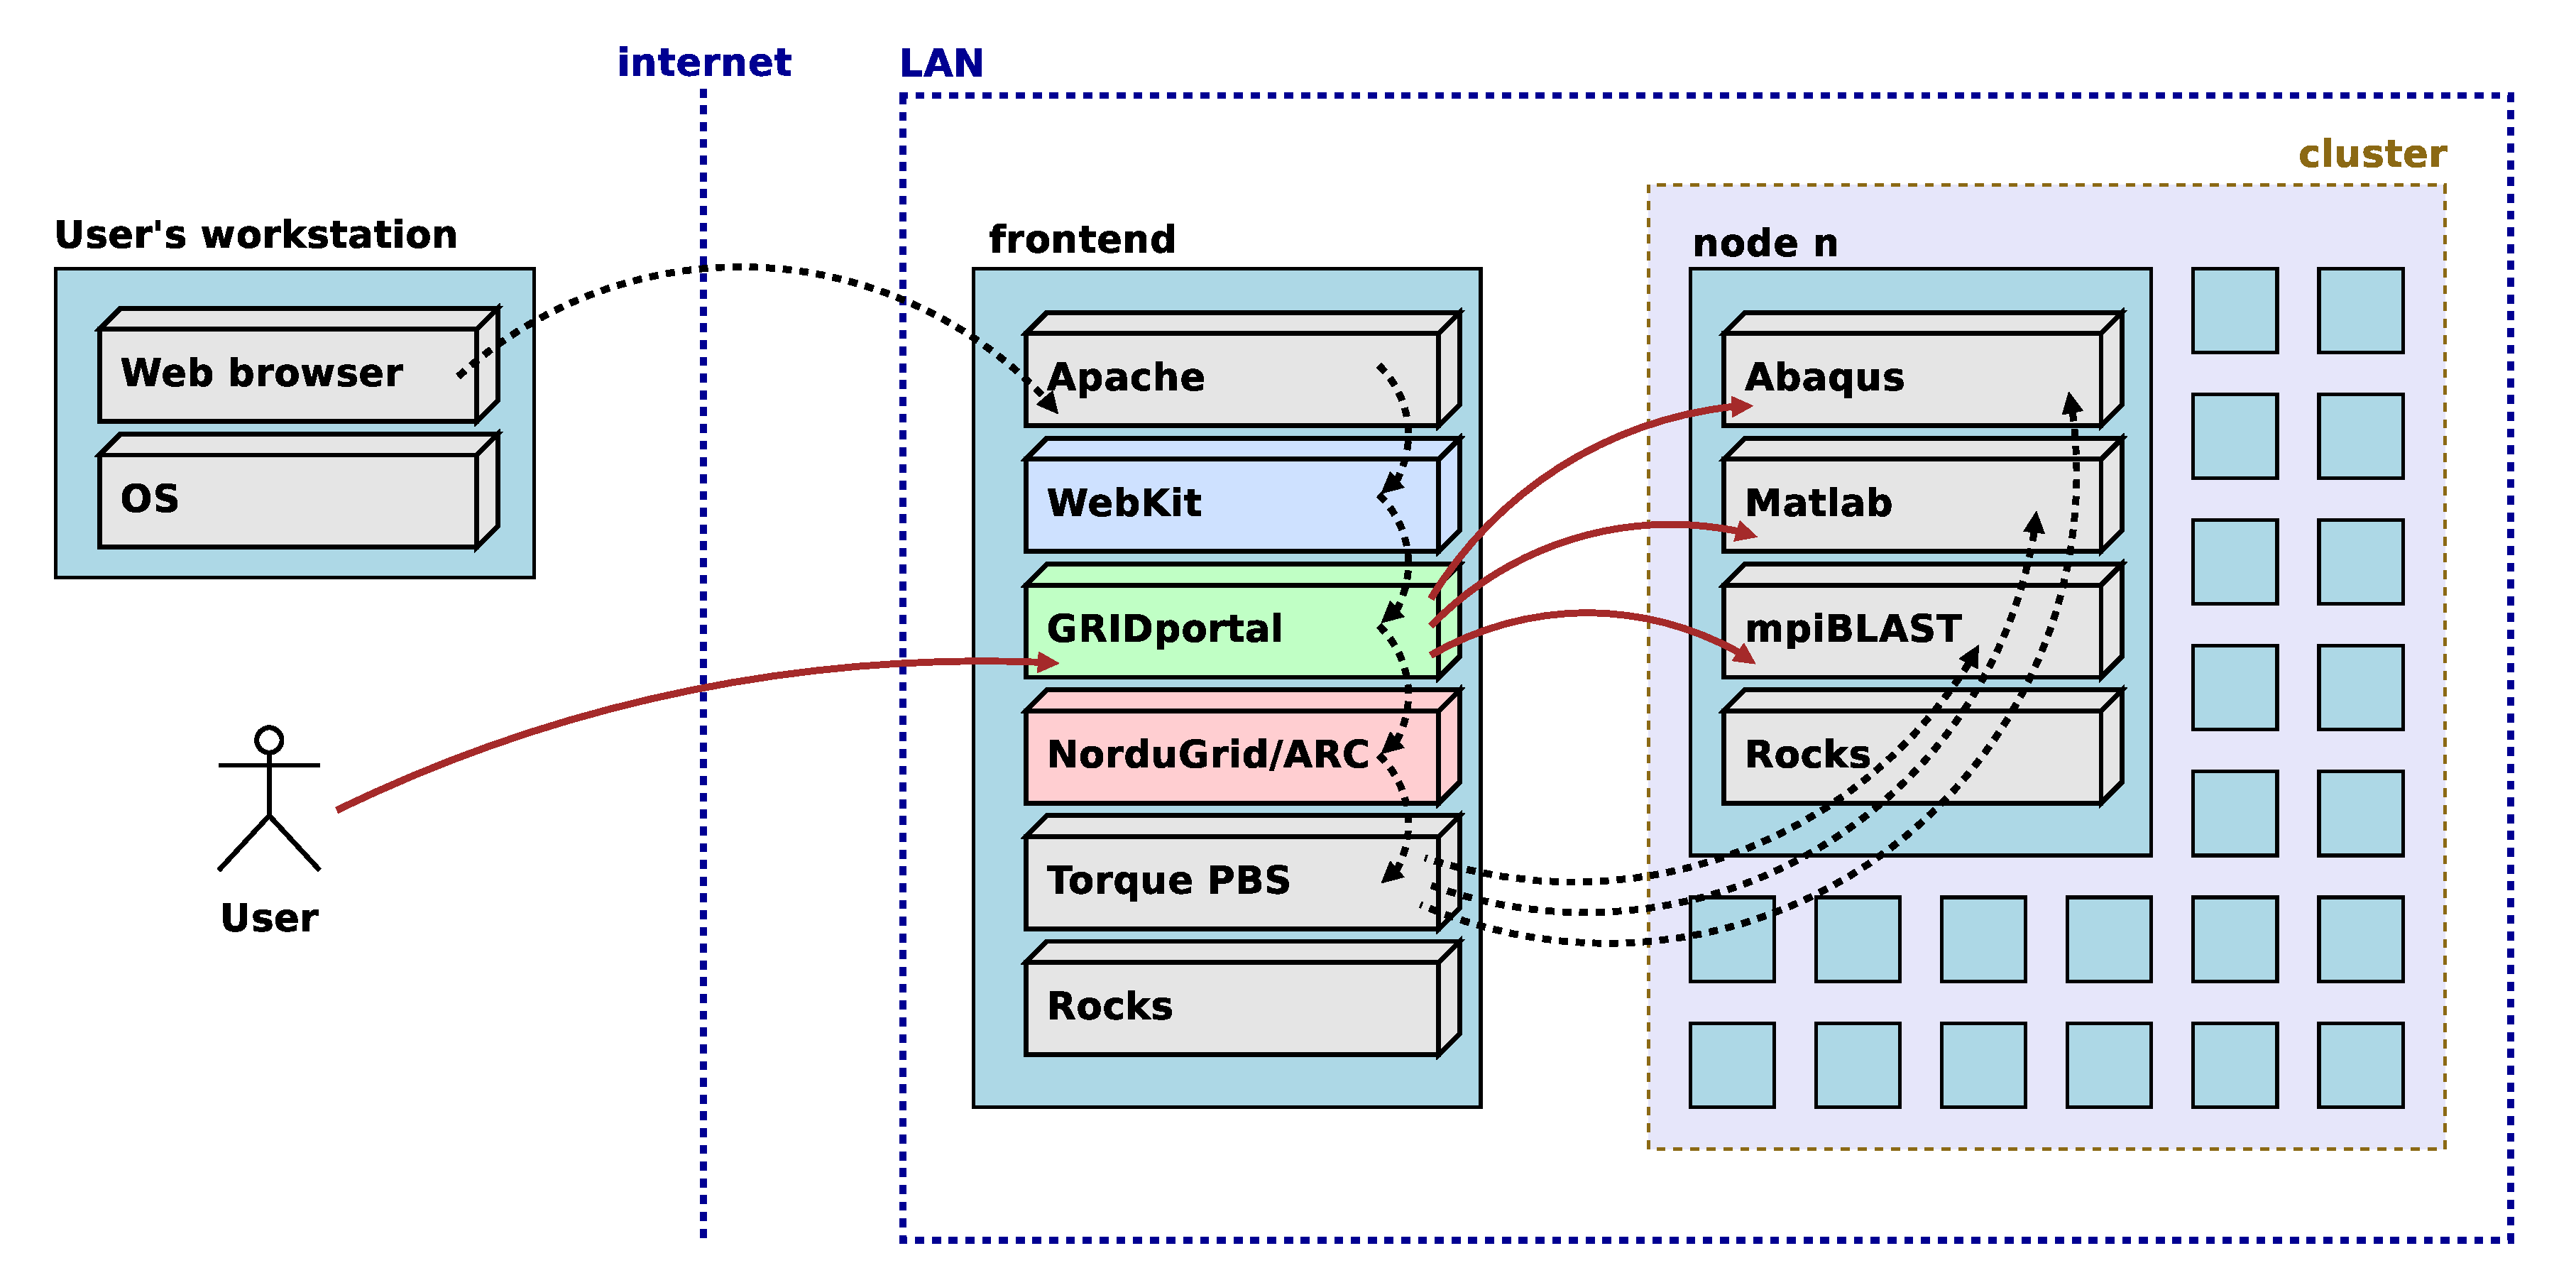
\includegraphics[width=1.0\textwidth]{physical.eps}
	\end{center}	
\end{frame}




\subsection{Authentication mechanism}


\begin{frame}
  \frametitle{Problem description}

	Nordugrid requires the following steps to be completed before a user can gain access to the network:
  \begin{enumerate}
  	\item The user must create a user certificate
	  \item The certificate must be signed by a Certificate Authority
	  \item The user must be accepted into a Virtual Organization
	  \item The user must generate a user proxy for every session
  \end{enumerate}
  \bigskip
  
  So how do we combine this with a web portal?
\end{frame}


\begin{frame}
  \frametitle{Proposed solution -- myProxy to the rescue}

	We deploy a client application for download to:
  \begin{enumerate}
  	\item Create a certificate
	  \item Mail certificate for signing
	  \item Register certificate with a myProxy server (a certificate store)
  \end{enumerate}
  \bigskip
  
  For every session: 
  \begin{enumerate}
  	\item The user logs in with a username/password, which is passed to the myProxy server
	  \item The portal receives a user proxy and passes it onto ARC
  \end{enumerate}
\end{frame}


\begin{frame}
  \frametitle{myProxy: a short description}

	{\bf Q.} So what is this myProxy thing?\\
	{\bf A.} myProxy is a certificate store, which can store user certificates in a "safe place". Since we wish to relieve the user of the burden of creating a user proxy for every session (as is the case with the command line interface), we transfer the responsibility of storing the certificate onto myProxy. The portal can then query myProxy for a user proxy whenever needed.
\end{frame}


\begin{frame}
  \frametitle{Authentication at a glance}

	\begin{center}
		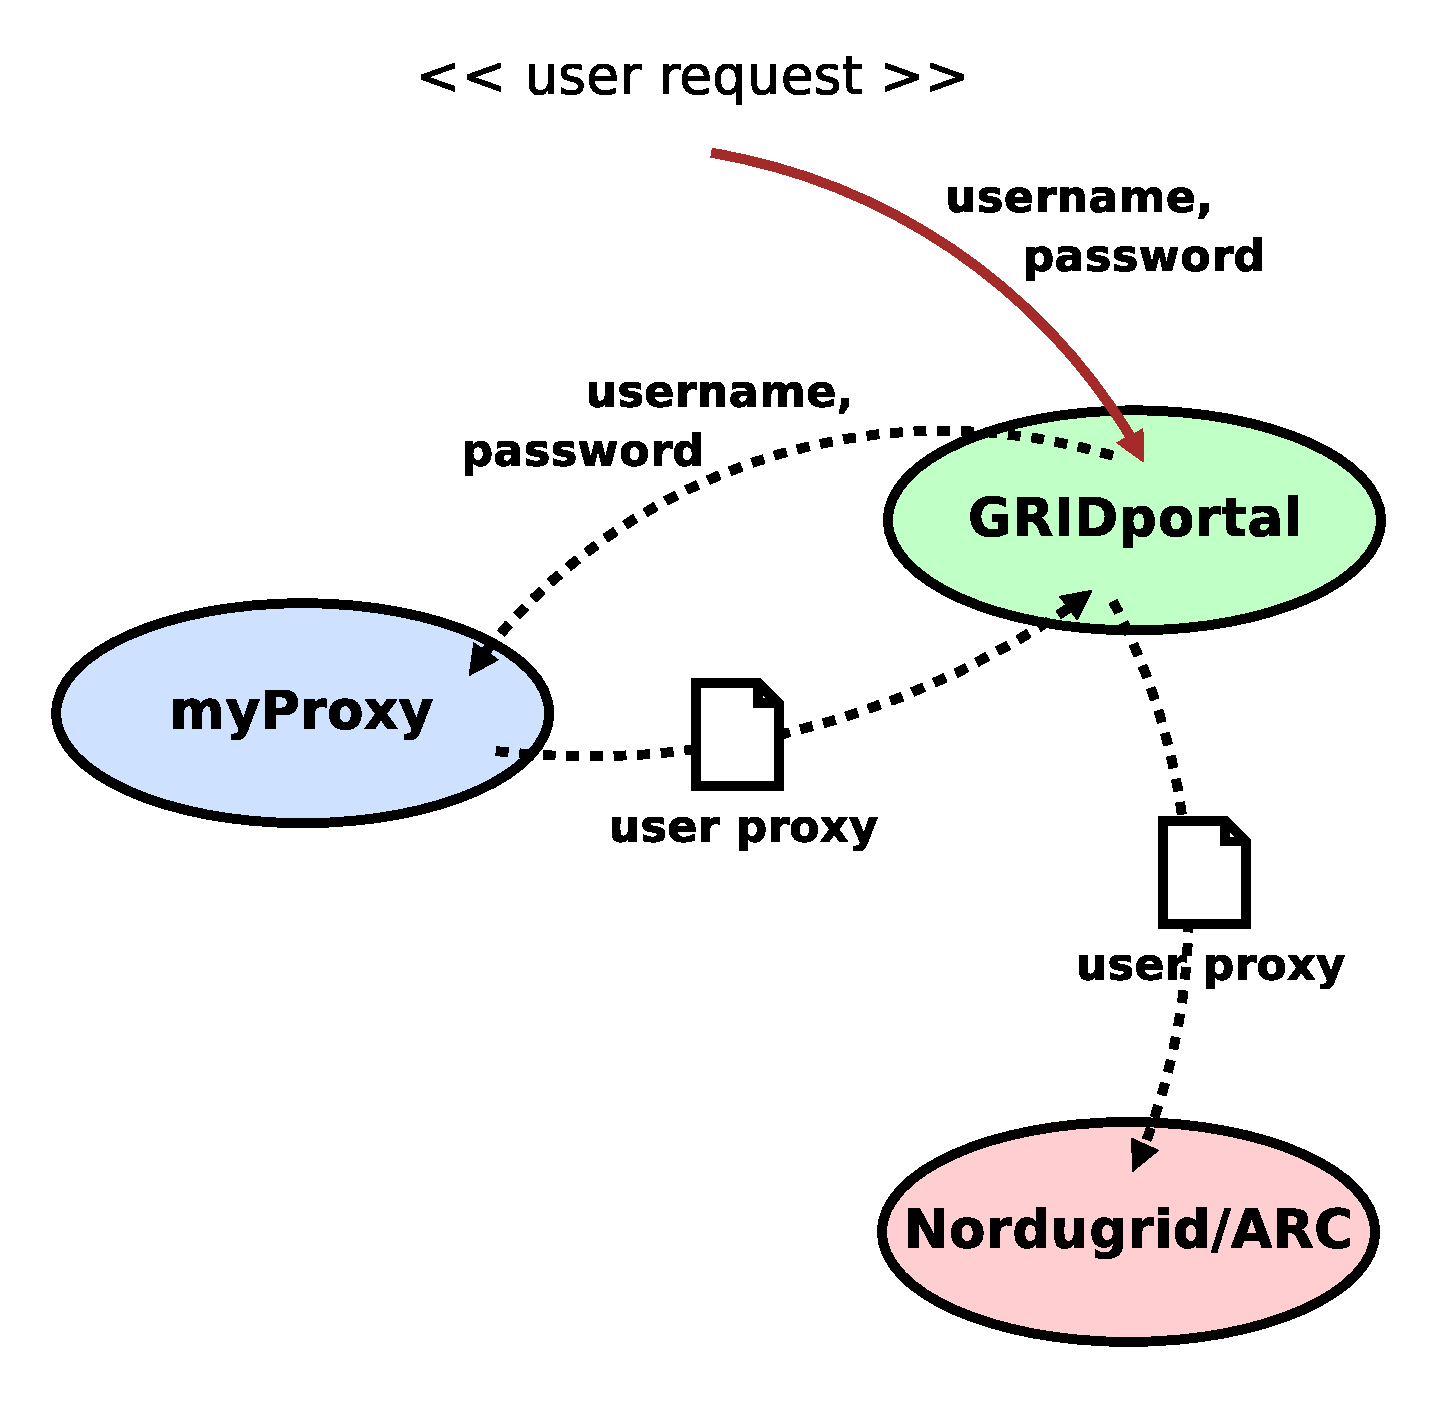
\includegraphics[width=0.6\textwidth]{myproxy.eps}
	\end{center}	
\end{frame}







\section{Applications on a GRID portal - BLAST}








\subsection{BLAST - an introduction}


\begin{frame}
  \frametitle{BLAST demystification -- a short description}

	BLAST
  \begin{enumerate}
  	\item compares biological sequences (written as text strings),
  	\item and yields results which describe the alignment between the sequences (the strings).
  \end{enumerate}
  {\footnotesize BLAST: <\url{http://www.ncbi.nlm.nih.gov/BLAST/}>}
\end{frame}


\begin{frame}
  \frametitle{BLAST demystification -- an example}

	The two sequences:
  \begin{enumerate}
  	\item a gene sequence from a specimen from the laboratory
  	\item a set of gene sequences from a known bacteria disease
  \end{enumerate}
	\bigskip
	
	The specimen sequence is compared to every sequence in the bacteria and for every alignment match (above a given threshold), a match is returned, along with a match score.
	\bigskip
	
	Depending on the results, there is something to be said for the presence of a sequence known in a common bacteria disease, in a specimen we take from a patient's blood.
\end{frame}


\begin{frame}
  \frametitle{BLAST vs speed -- an N:M problem}

	A typical BLAST query involves comparing
  \begin{enumerate}
  	\item many specimen sequences (anything from one sequence to millions of sequences)
  	\item to a sizeable database of sequences (e.g. 4GB)
  \end{enumerate}
  \bigskip
  
  The BLAST algorithm, comparing sequences one by one, is characterized as {\it embarassingly linear}, so a speed boost could be possible through symmetric processing.
\end{frame}


\begin{frame}
  \frametitle{The solution: mpiBLAST}

	mpiBLAST, built with the Message Passing Interface (MPI), is a parallellized flavor of BLAST, designed for use on a cluster. It
  \begin{enumerate}
  	\item divides the database into equal segments,
  	\item distributes each segment onto a node,
  	\item performs BLAST search on each node in parallell,
  	\item and merges the results from each node into a common result set.
  \end{enumerate}	
\end{frame}


\begin{frame}
  \frametitle{Evaluating mpiBLAST}

  {\it "Database segmentation yields near linear speedup of BLAST in most cases and super-linear speedup in low memory conditions."}\\  
	{\footnotesize The Design, Implementation, and Evaluation of mpiBLAST\\
	A. Darling, L. Carey, and W. Feng}\\
	{\scriptsize ClusterWorld Conference \& Expo in conjunction with the 4th International Conference on Linux Clusters: The HPC Revolution 2003, San Jose, CA, June 2003.}
\end{frame}





\subsection{BLAST at norgrid.ntnu.no}

\begin{frame}
  \frametitle{Creating a BLAST job with GRIDportal}

	\begin{center}
		\includegraphics[width=0.7\textwidth]{portal_createblast.png}
	\end{center}	
\end{frame}


\begin{frame}
  \frametitle{BLAST with large data sets}

	Depending on the number of matches in a BLAST query, the result file may become rather large.
	
	\begin{center}
		\includegraphics[width=0.8\textwidth]{blast_filesize.png}
	\end{center}		
\end{frame}


\begin{frame}
  \frametitle{GRIDportal vs large data sets}

	The portal is web-based, uploading/downloading of input/output files is over HTTP. On slow links, the transfer is likely to suffer from bad connectivity, network congestion etc. {\it And there is no resume function for interrupted transfers.}
	\bigskip
	
	Thus, heavy BLAST users are better off using the command line interface. {\bf In general, the portal is well suited for jobs with heavy processing but small input \& output files.}
\end{frame}








\appendix
\section<presentation>*{\appendixname}
\subsection<presentation>*{References}

\begin{frame}
  \frametitle{Links}

  \begin{itemize}
  	\item GRIDportal project website <\url{http://gridportal.dynalias.org/}>
  	\item GRIDportal deployment site <\url{http://norgrid.ntnu.no/gridportal/}>
  \end{itemize}
  \bigskip

  \begin{center}
  Thank you for your attention!
  \end{center}
\end{frame}




\end{document}


